\documentclass{article}
% \documentclass{beamer}
% \usetheme{Madrid}

%------------------------------
% used for href/url
\usepackage{hyperref}


% used for math fomulas
\usepackage{amsmath}

% used for pictures
\usepackage{graphicx}
\usepackage{subcaption}
\usepackage{float}

% used for codes
\usepackage{listings}
\lstset{
  basicstyle=\ttfamily\footnotesize, % Set your code to be drawn with a monospaced font
  breaklines=true, % Enables line breaking
  frame=single % Adds a frame around the code
}

% used for Graph
\usepackage{adigraph}

% used for Bayesian Network
\usepackage{tikz}
\usetikzlibrary{bayesnet}

%------------------------------
% TODO 
\tolerance=10000
\emergencystretch=\maxdimen
\hyphenpenalty=10000
\hbadness=10000


\usepackage{silence}
\WarningFilter{latex}{Overfull \hbox}

%------------------------------



\title{MK's Latex Examples}
\date{2024-02-15}
\author{Yonggang Chen (Michael)}

\begin{document}
  \pagenumbering{gobble}
  \maketitle
  \newpage
  \pagenumbering{roman}


  % ----------------------------------------
  \tableofcontents
  \newpage


  % ----------------------------------------
  {\Huge Hello World! @ \href{https://www.auburn.edu/}{AU Homepage} }

  {\huge ... }

  {\huge Let's begin our learning here }
  {\large \url{https://latex-tutorial.com/tutorials/first-document/} }
  \newpage

  % ----------------------------------------
  \section{Various Bullets}
  \begin{enumerate}
    \item One
    \begin{enumerate}
        \item Two
        \item Three
        \item Four
    \end{enumerate}
    \item Five
      \begin{itemize}
        \item X
        \item Y
        \item Z
      \end{itemize}
    \item Six
  \end{enumerate}
  \newpage


  % ----------------------------------------
  \section{Writing Formulas}
  \subsection{Equation - ONLY support one formula per line}
  \begin{equation}
    formula 1: f(x) = x^2   ----
    formula 2: \prod_{2}^{n}
  \end{equation}

  \subsection{Align - support MULTIPLE formulas in the same block}
  NOTE: need use package amsmath to enable Align 
  \begin{align*}
    f(x) &= x & 2 \\
    g(x) &= \frac{1}{x} \\
    F(x) = f(x) + g(x) &= \int_{a}^{b} \frac{1}{3}x^3 \\
    W(x) &= \frac{1}{\sqrt{x}} + \frac{1}{\sqrt[3]{y}} \\
    Z(x) &= \left( 3 + 2 \right) * 2
  \end{align*}
  \subsubsection{}
  So which one, align or equation, will you use?


  \subsection{Inline math}
  The form is used for $ f(x) = x^ 2 $ or $\lambda$, so you can easily to use them. 
  https://github.com/LucaCappelletti94/adigraph
  \subsection{Matrics}
  $
  \left[
  \begin{matrix}
    3 & 2 \\
    9 & 4 & x
  \end{matrix}
  \right]
  $

  \newpage


  % ----------------------------------------
  \section{Embedding Pictures/Figures}

  \subsection{One figure}
  NOTE: need to use package graphicshttps://github.com/LucaCappelletti94/adigraph to enable figure

  \begin{figure}[h!]
    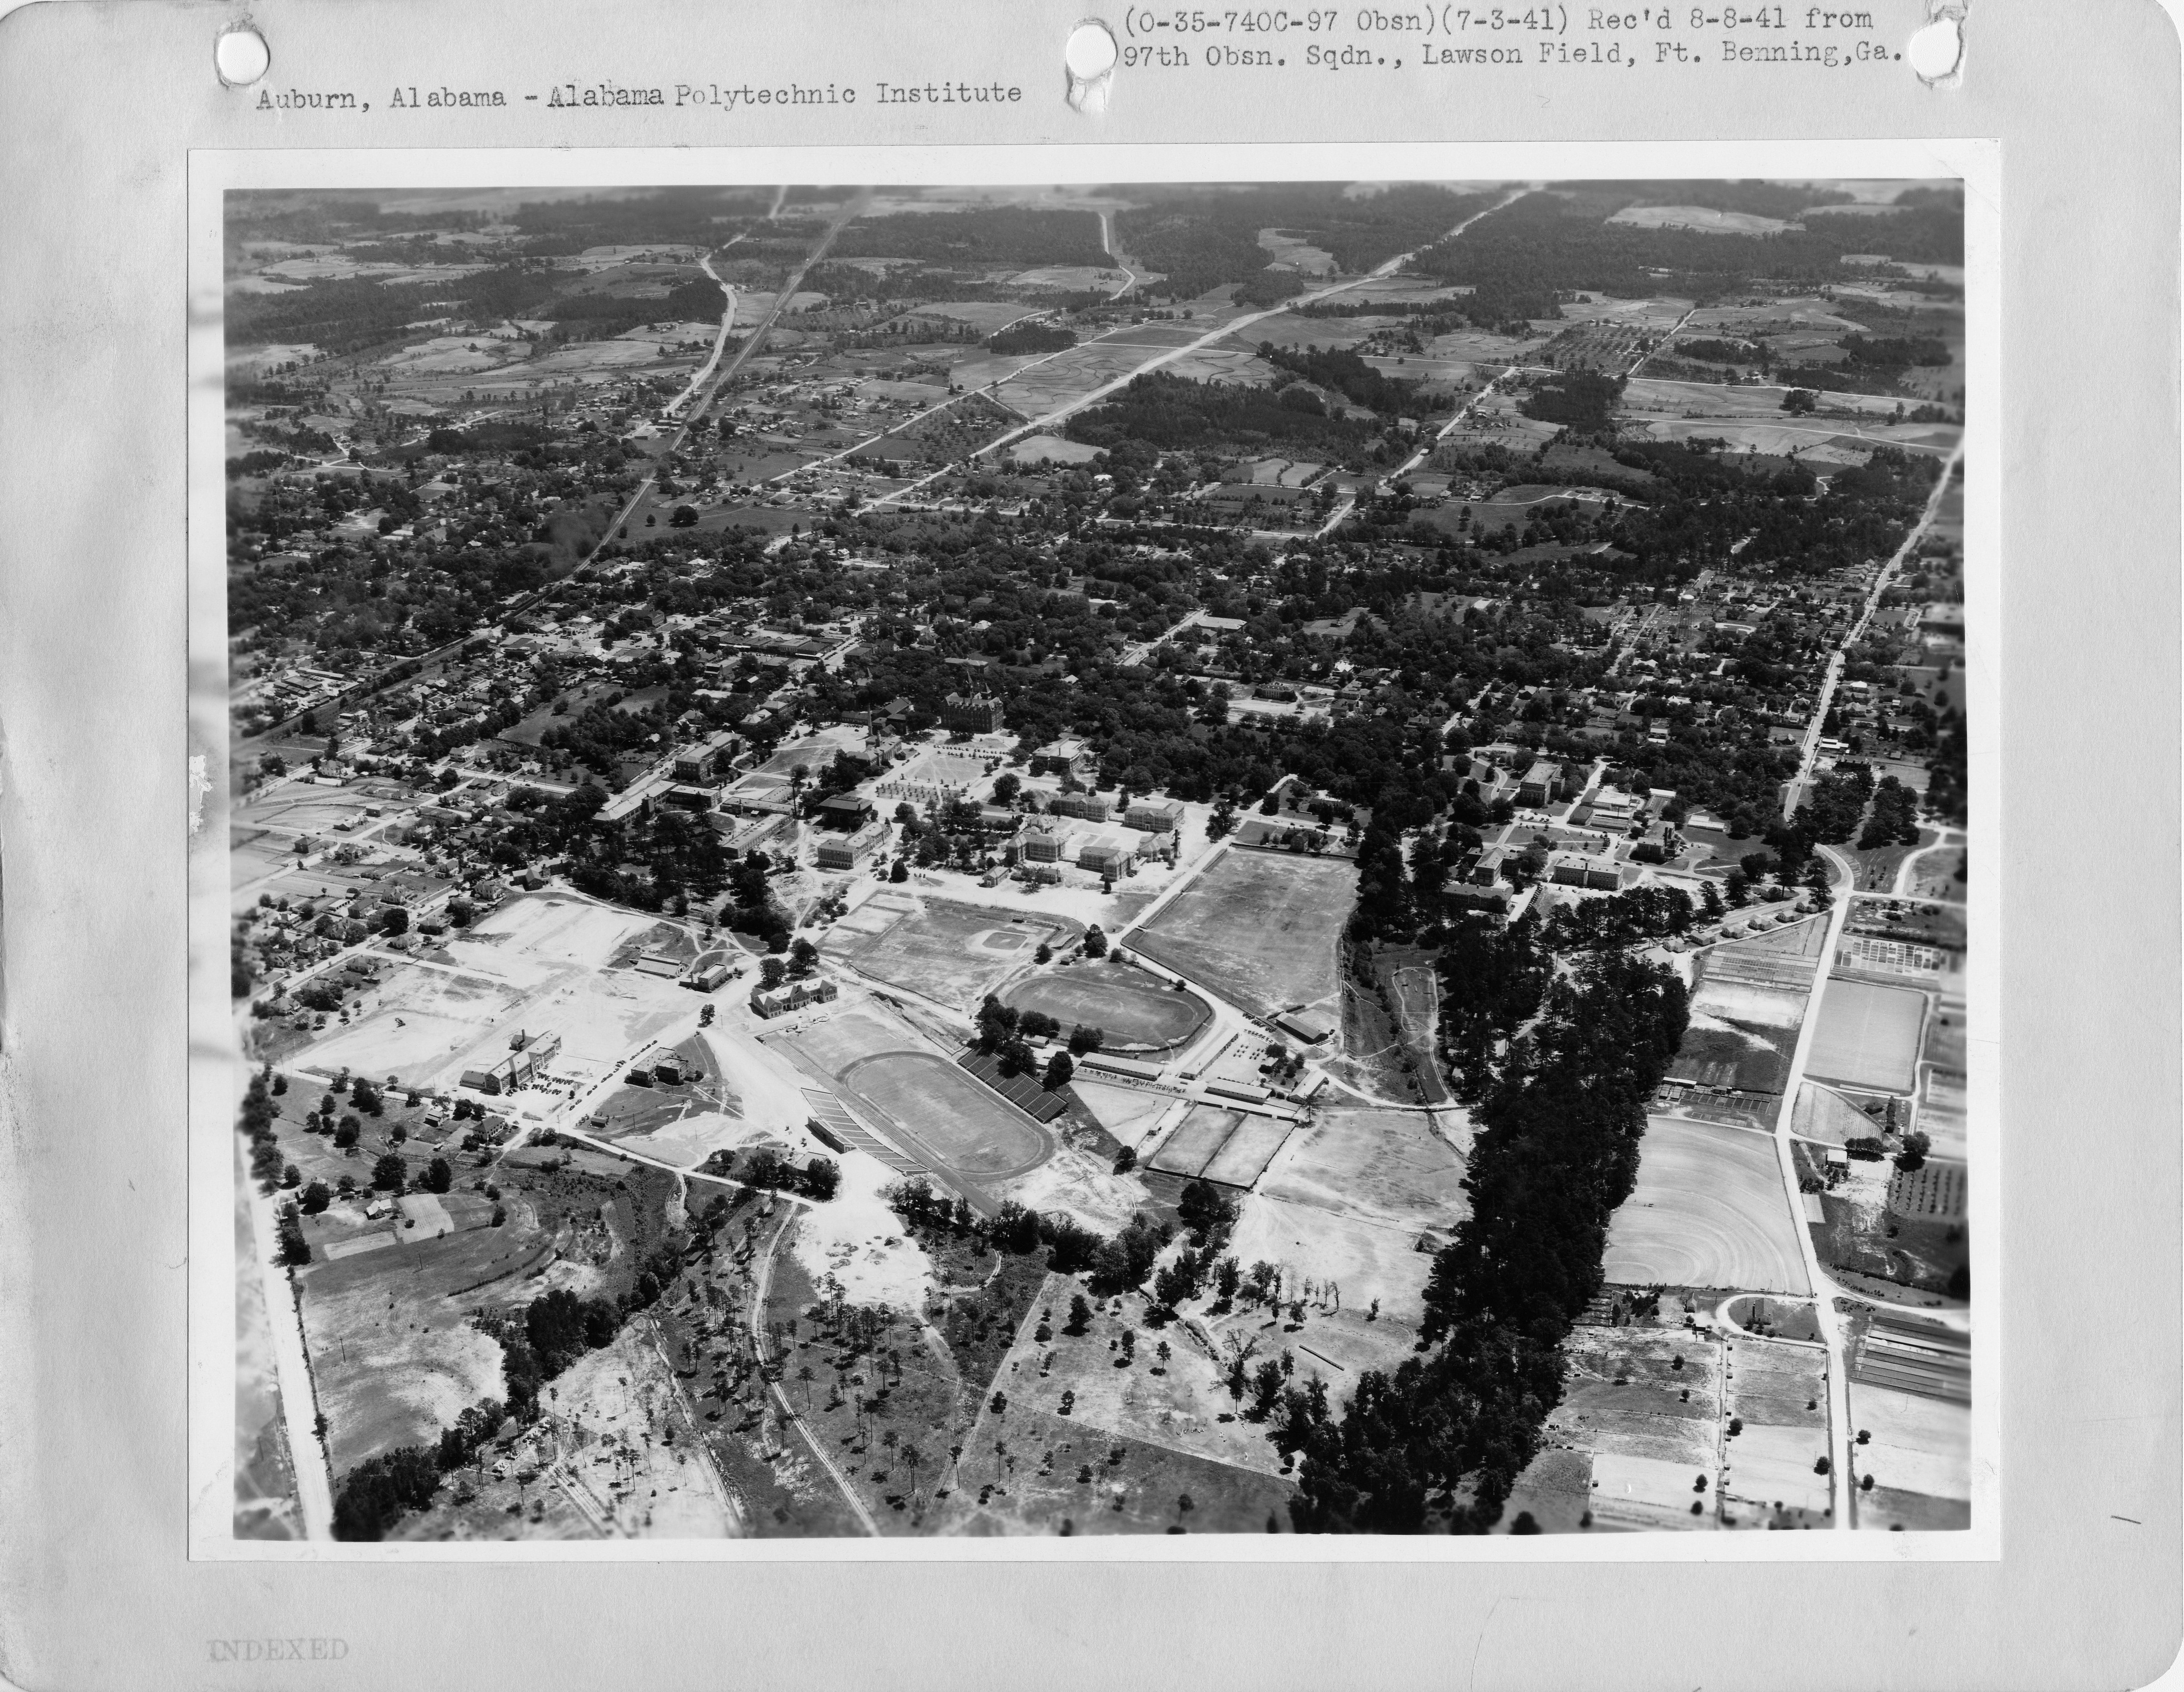
\includegraphics[width=\linewidth]{auburn_01.jpg}
    \caption{Auburn Campus}
    \label{fig:au01}
  \end{figure}

  \subsection{Multiple figures}
  NOTE: need to use package subcaption to enable Multiple figures.
  Here are figures:
  \begin{figure}[H]
    \centering
    \begin{subfigure}[b]{0.4\linewidth}
      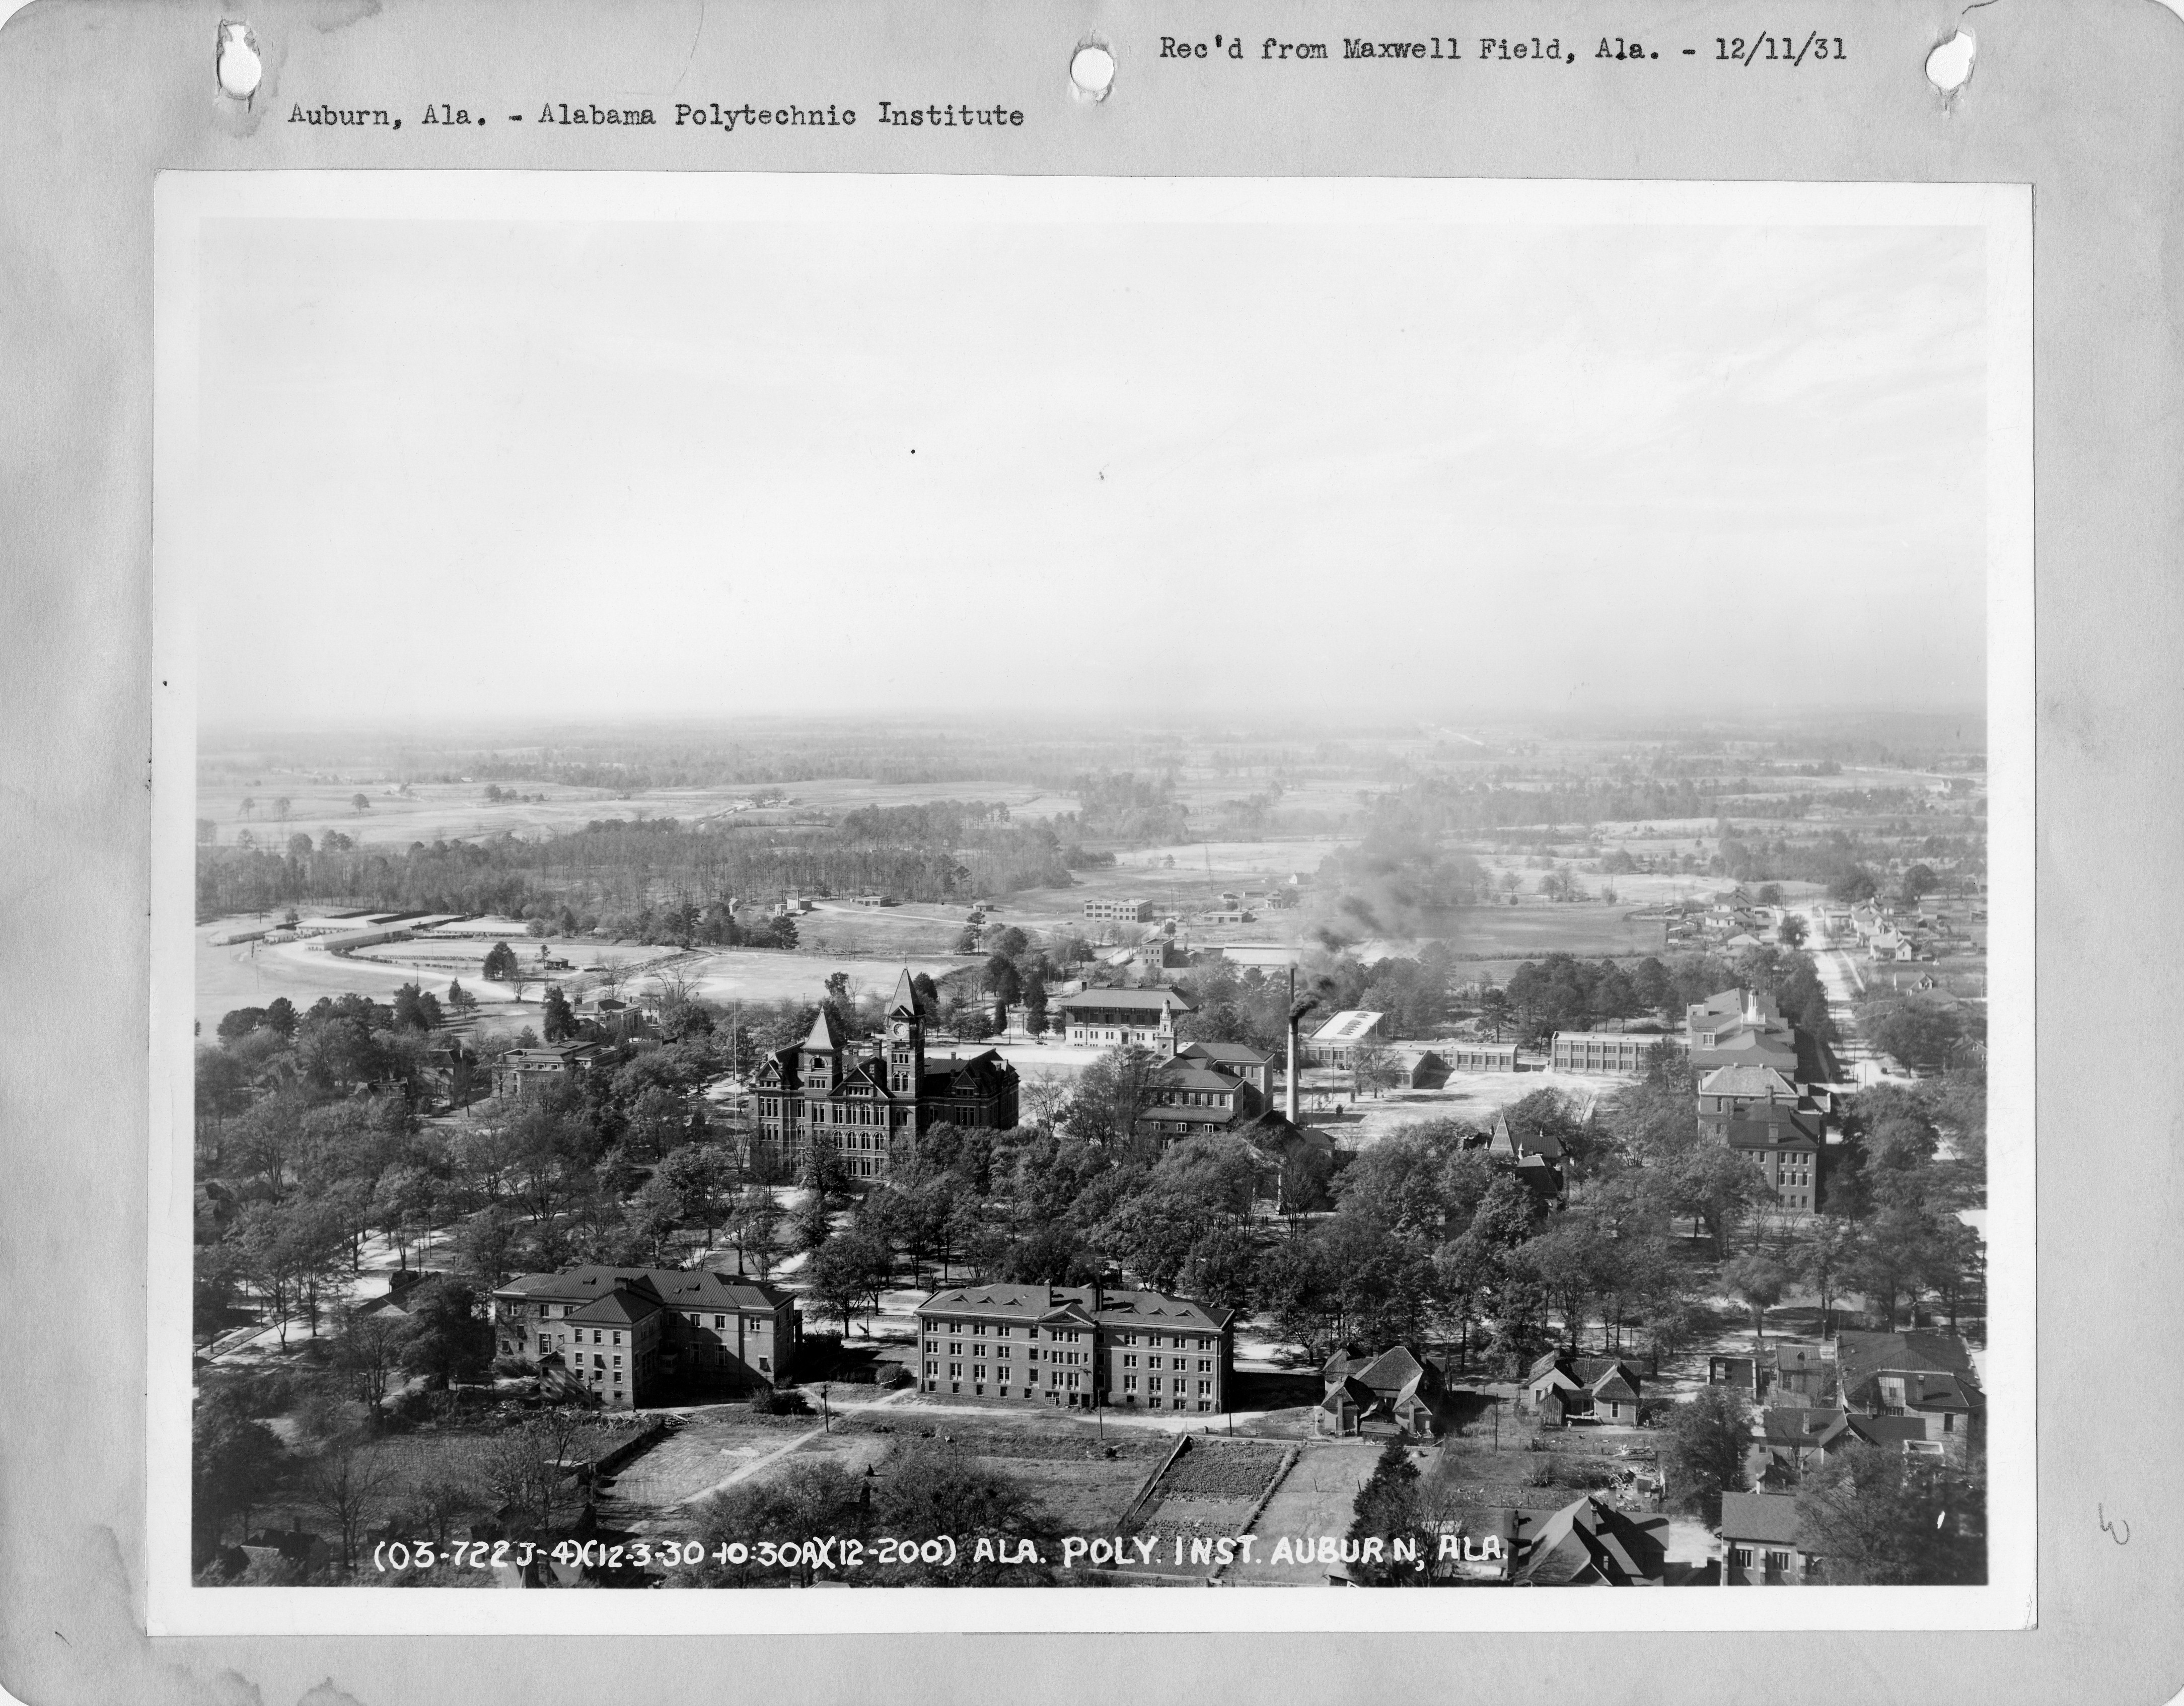
\includegraphics[width=\linewidth]{auburn_02.jpg}
      \caption{Auburn Overview}
    \end{subfigure}
    \begin{subfigure}[b]{0.4\linewidth}
      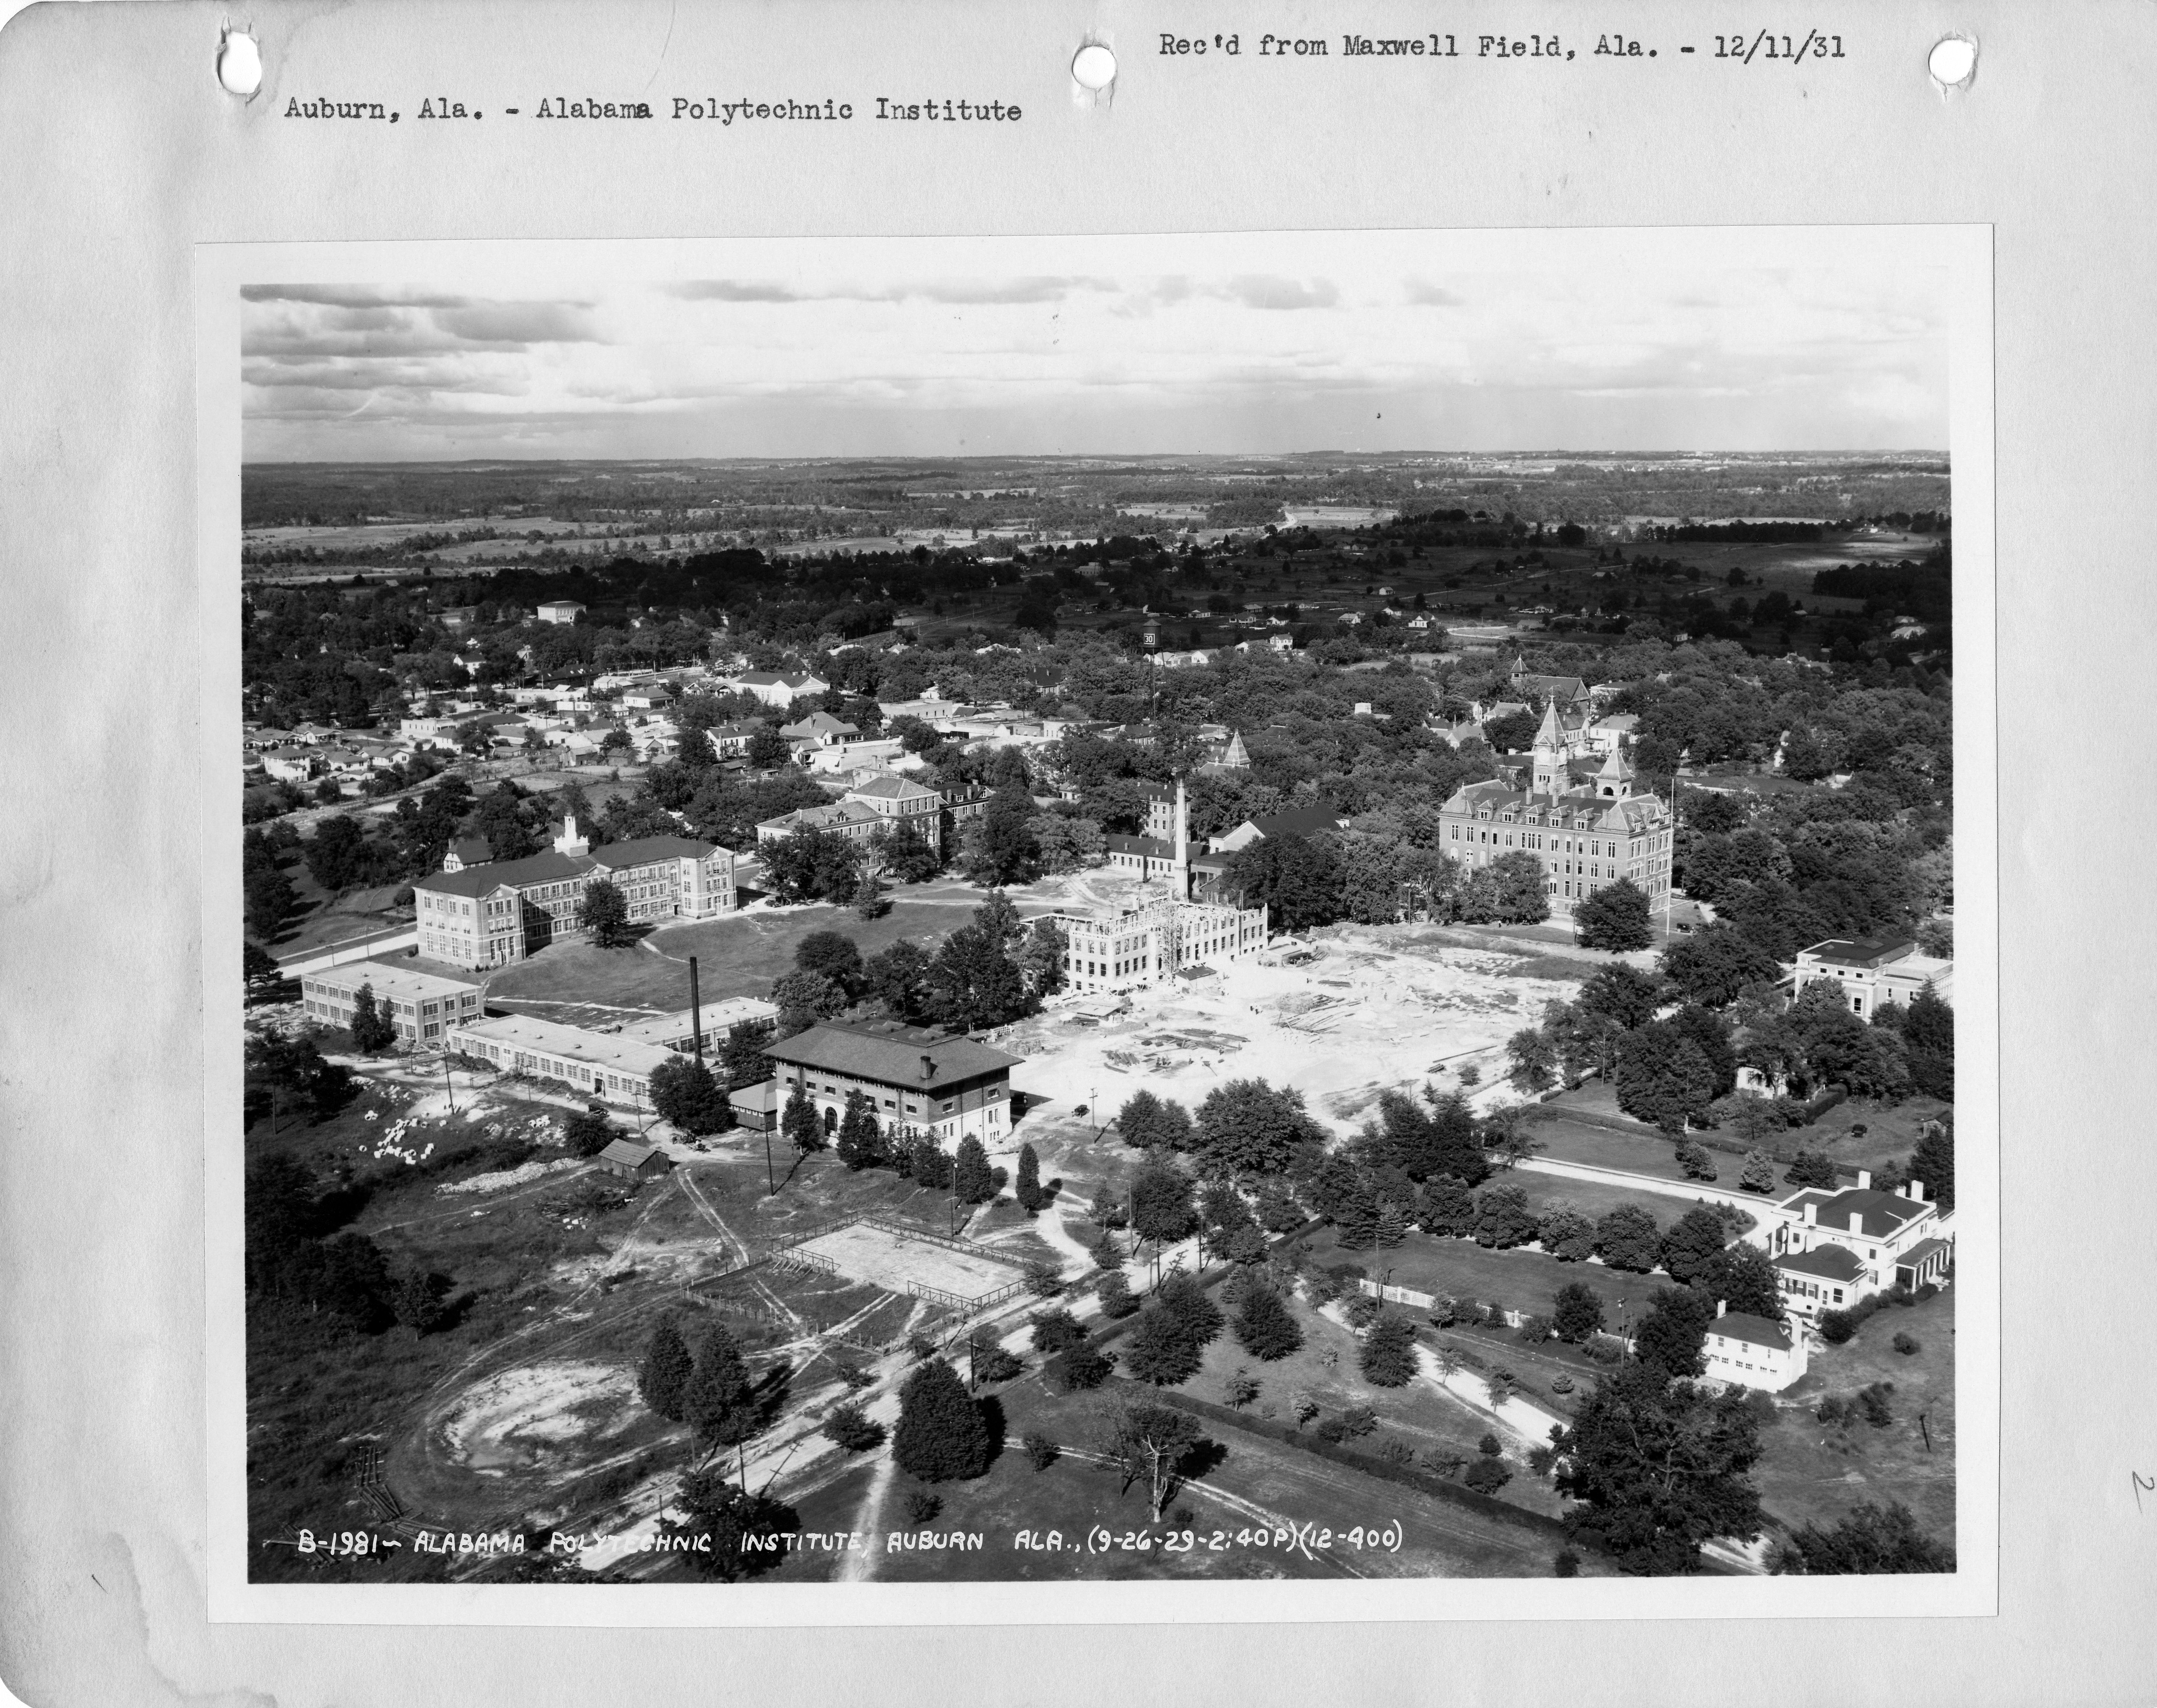
\includegraphics[width=\linewidth]{auburn_03.jpg}
      \caption{Auburn Buildings}
    \end{subfigure}
    \caption{Two Auburn Old Pictures}
    \label{fig:twoPic}
  \end{figure}

  \subsection{Use float and H}
  Use package float and attribute H to strictly fix the pictures' posisiton to HERE.

  \begin{lstlisting}[caption={An Example}]
    \usepackage{float}
    ...


    \begin{figure}[H]
      ....
    \end{figure}

    
  \end{lstlisting}
  \newpage


  % ----------------------------------------

  \section{Drawing Bayesian Network and Graph}
  \subsection{Use pagckages: tikz and bayesnet}
  Use 2 packages: tikz and bayesnet to draw Bayesian Network chat.
  \break

  Type 1:
  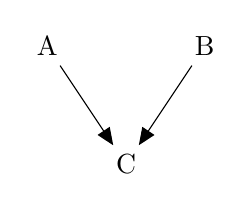
\begin{tikzpicture}
  \node (A) at (0,0) {A};
  \node (B) at (2,0) {B};
  \node (C) at (1,-1.5) {C};
  \draw[->] (A) -- (C);
  \draw[->] (B) -- (C);
  \end{tikzpicture}


  Type 2:
  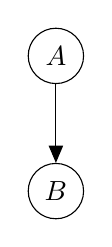
\begin{tikzpicture}
  \node[latent] (A) {$A$};
  \node[latent, below = of A] (B) {$B$};
  \edge {A} {B};
  \end{tikzpicture}
  \iffalse
  \fi
  
 
  \subsection{Use pagckages: adigraph}

  \NewAdigraph{myAdigraph}{
    s:0,0;
    1:2,2;
    3:2,-2;
    2:6,2;
    4:6,-2;
    t:8,0;
}{
    s,1:25;
    s,3:25;
    3,4:25;
    1,2:35;
    2,t:20;
    4,t:30;
    3,1:10;
    4,2:10;
    2,3:15::near start;
    4,1:5::near start;
}
\myAdigraph{}

\newpage


% --------------------------------------
\section{Using packages}
Packages are like plugins to extend the Latex' capabilities. Some common commands are listed here.

\begin{lstlisting}[language=bash, caption={tlmgr commands and etc}]
tlmgr list --only-installed   # show installed packages

tlmgr search <package-name>   # search a packages
tlmgr info <package-name>     # show a package's intro, no matter installed or not
tlmgr install <package-name>  # install a new packages

tlmgr update --self --all     # update package index

kpsewhich article.sty         # locate a package's .sty file

# env variables can define additional directories to be searched. 
echo $TEXMFHOME $TEXMFLOCAL $TEXMFSYSCONFIG 
\end{lstlisting}
\newpage


% --------------------------------------
\section{Generate Slides}
Use the package beamer to generate a pdf file of slides from an article


\begin{lstlisting}[caption={Changes in .tex file}]
  % \documentclass{article}
  \documentclass{beamer}
  \usetheme{Madrid}
\end{lstlisting}

% --------------------------------------
\end{document}